\documentclass[conference]{IEEEtran}
\usepackage[center]{caption}
\usepackage{wrapfig}
\usepackage{textcomp}
\usepackage{graphicx}
\usepackage{mathrsfs}
\usepackage{subcaption} 
\usepackage{esint}

\graphicspath{ {./images/} }
\providecommand{\keywords}[1]{\textbf{\textit{Keywords ---}} #1}

\begin{document}
\title{Hyperparameter Tuning in LSTM }
\author{
    \IEEEauthorblockN{Prabesh Poudel\IEEEauthorrefmark{1},
        Prabesh Pathak\IEEEauthorrefmark{2},
        Binish Koirala\IEEEauthorrefmark{3},
        Bishal Neupane\IEEEauthorrefmark{4},
        Robert C. Green II\IEEEauthorrefmark{5}
    }
    \IEEEauthorblockA{
        Department of Computer Science\\
        Bowling Green State University\\
        Bowling Green, Ohio, 43403\\
        pprabes@bgsu.edu\IEEEauthorrefmark{1},
        ppathak@bgsu.edu\IEEEauthorrefmark{2},
        binishk@bgsu.edu\IEEEauthorrefmark{3},
        bneupan@bgsu.edu\IEEEauthorrefmark{4}, 
        greenr@bgsu.edu \IEEEauthorrefmark{5}
    }
}

% make the title area
\maketitle

\begin{abstract}
Neural network models such as LSTM have several hyperparameters that substantially affect their performance. But finding and tuning the optimal hyperparameters in a high dimensional space is not a trivial task. Our paper implements four search methods to tune the hyperparameters in LSTM networks. First, we select four hyperparameters: number of hidden units, learning rate, number of epochs and, input length. Second, we draw comparisons among the methods used. The paper uses the IMDB movie review dataset which contains $50,000$ reviews and is listed on the official tf.keras website. Among the methods used, our approach to the genetic algorithm yielded the best results with the area under the precision-recall curve (AUC) of $0.946$.
\end{abstract}

\keywords{LSTM, Hyperparameters, Tuning, Genetic Algorithm}
\section{Introduction}
Recurrent Neural Networks (RNNs) are a class of artificial neural networks that have hidden states and allow previous outputs to be used as inputs.
They are popular in the fields of Natural Language Processing and Speech Recognition. 
LSTM (Long Short Term Memory) network \cite{lstm} is a special kind of RNN that is capable of learning long term dependencies. 
We intend to explore the effects of hyperparameters in LSTM.
LSTM has a broad range of hyperparameters such as learning rates, number of hidden units, input length, batch sizes, and so on.
The selection and optimization of hyperparameters often make the difference between the mediocre and the state-of-the-art performance \cite{hutter}.

The learning rate determines the size of the step that the model takes in each update of its parameter while converging and minimizing a loss function. The number of hidden units is the dimension of the hidden state of the LSTM cell. It represents the model's learning capacity. Input length refers to the number of input timesteps. In our context, the input length of $l$ refers to the first $l$ number of words of a movie review the LSTM sees before making a correct prediction. We try to see if the LSTM doesn't need the whole sequence to make a correct prediction and determine the optimal value for this length.  

Several search algorithms are used for tuning hyperparameters. Grid search is a popular technique that computes the optimum values of hyperparameters. This is an exhaustive search that is performed on a search space of manually defined parameters and evaluates the model for each combination to identify the best results. In grid search, the number of evaluations increases exponentially with an additional parameter because of the dimensionality. Using the grid search can be computationally expensive as the combination of the parameters grows.

One of the techniques to deal with the computational cost of grid search is random search. It generates a random combination of hyperparameters from a range of values to find the optimal solution for the built model. Random search is found to be more efficient than a grid \cite{random} since it solves the curse of dimensionality. A limitation of random search is that hyperparameters chosen in each iteration are completely random. As the process of choosing hyperparameter does not take into account previous outcomes, it does not necessarily lead us closer to the optimal solution.

Bayesian optimization is a statistical approach which overcomes this issue by guiding the model to probably choose a better set of hyperparameter in next iteration. This approach takes into account the past selections and the corresponding performance to make a prediction on which set of hyperparameters will yield better results and tries them in the next iteration. It works by building a statistical model of the surrogate function from the hyperparameter values and then choosing parameters that minimize the loss. Finally, these selected samples are evaluated by the real objective functions.


The genetic algorithm is an evolutionary technique inspired by the process of natural selection and survival of the fittest. For the initial generation, the population pool consists of several random individuals. Individuals who perform better have a higher chance of having their characteristics passed onto the next generation. Based on a function, fittest new individuals are identified and added to the pool for the upcoming generation in each iteration. After several iterations, we converge on the solution.

We work with four hyperparameters. We choose not to use batch size because it has no significant effect on performance \cite{batch}. This paper expects to answer the following questions: \begin{itemize}
\item  RQ1: How do the hyperparameter tuning techniques compare with each other?
\item  RQ2: Which set of above-mentioned hyperparameters yields the best results for LSTM?

    
\end{itemize}
We use random search, Bayesian optimization, and genetic algorithm to get highly performant hyperparameters. 
Then we apply a grid search on the hyperparameters obtained from the three techniques listed above. 
Our key contributions include :  
\begin{itemize}
    \item Tuning four hyperparameters in LSTM for IMDB dataset: learning rate, number of hidden units, input length and number of epochs.
    \item Implementation of four different methods to find the optimal hyperparameters: Random search, Bayesian optimization, Genetic Algorithm, and Grid Search.
    \item Implementation of Grid Search to decide the final best hyperparameter. First, we use a Genetic Algorithm to find the top $3$ models. Then we use one each(best ones) from Random and Bayesian method to fit a total of $5$ models in the grid search to find the best one.
\end{itemize}
The rest of the paper is presented as follows. In Section II, we discuss the background and related works in the field of hyperparameter tuning. In Section III, we explain the methodology and implementation of our work. We present, evaluate, and discuss the result in Section IV. We conclude our study and discuss potential future works in Section V.

\begin{figure}
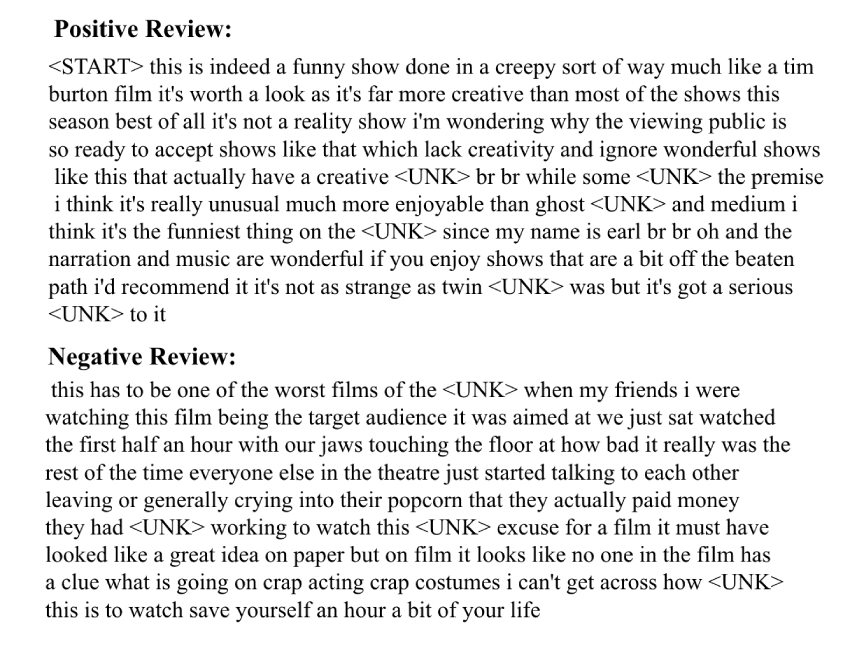
\includegraphics[width=0.5\textwidth, height=11cm, keepaspectratio]{posnegtypes.png}
\caption{Examples of two classes of reviews from the IMDB dataset}
 \label{fig:eg}
\end{figure}

\section{Background}
\subsection{Dataset Description}
We used IMDB Review dataset which was also used by Mass et al.\cite{imdb}. The dataset consists of $50,000$ reviews from IMDB with no more than $30$ reviews per movie including an approximately equal number of positive and negative reviews. The dataset is readily available with tenserflow.keras.dataset. The mean length a review in the dataset is $234.75$ words and the standard deviation is $172.91$. Examples of reviews can be seen in Figure \ref{fig:eg}. A review belongs to either a positive or negative class. Only the top $5000$ frequently used words are retained and the remaining words are labeled as $<$UNK$>$ and do not contribute to the model.

\subsection{Related Works}
Several methods have been used for hyperparameter tuning to optimize accuracy and performance\cite{methods} of machine learning models. One of the most popular methods is the grid search. Grid search exhaustively generates candidates from a grid of parameter values. Random search \cite {random,odyssey} is more efficient and deals with the computational issues of grid search. Random search replaces the exhaustive enumeration of all combinations by selecting them randomly. Since random search does not adapt its behavior based on previous outcomes we use Bayesian Optimization\cite{bayesian} method that helps us to use the past evaluation results to choose the next values to evaluate. Similarly, we also use the genetic algorithm to aid our hyperparameter optimization.

The work that is closest to our approach is work from Reimers and Gurevych\cite{optimal}. In their work, the authors evaluate the importance of different network design choices and hyperparameters for five common linguistic sequence tagging tasks and state that the choice of certain hyper parameters have high impact on achieved performance. They worked with tuning eleven hyperparameters whereas we work with four hyper parameters. Our approach is similar to theirs but we also had additional approach with genetic algorithms to optimize hyperparameters.

Melis et al.\cite{melis} use  black-box technique\cite{blackbox} to optimize hyperparameters  by comparing the relative performance of language modeling architectures based on LSTMs. A similar approach is also followed by Merity, McCann, and Socher \cite{merita} to explore model and setting. They conclude that underlying LSTM architecture with tuned hyperparameters can be highly effective compared to complex custom architecture.

Bergstra et al.\cite{methods} used random search and two novel greedy sequential methods to optimize hyperparameters based on the expected improvement criterion and present the optimized hyperparameters on the task of s on tasks of training neural networks and deep belief networks (DBNs). They found the random search to be sufficiently efficient for learning neural networks and the sequential algorithms yielded significantly better results for DBNs.

Hutter, Lucke and Thieme \cite{hutter} discuss the automated optimization of hyperparameters including the mechanisms for feature selection, preprocessing and algorithm selection and develop novel algorithms with fewew hyperparameters.

Bengio used gradient-based algorithms to select many hyperparameters simultaneously using the gradient of the model selection criterion with respect to the hyperparameters\cite{bengio}.

Thronton et al.\cite{weka} leveraged on the innovations of bayesian optimization to select the learning algorithms and to set appropriate hyperparameters to them and achieve the improved performance using the Auto-WEKA tool.

Li et al. \cite{asha} introduced a simple and robust hyperparameter optimization algorithm called ASHA, that exploits parallelism and early stopping to solve large scale hyperparameter optimization.

\section{Methodology}

Our methodology consisted of random search, Bayesian optimization, genetic algorithm, and grid search. We divide the dataset into training, validation, and test set. Training set($20,000$) and validation set ($5,000$) consists a total of $25,000$ labeled reviews whereas test set has remaining $25,000$ labeled reviews. The dataset consist of movie reviews and its labels consist of $0$ and $1$, where $0$ means a negative review and $1$ stands for a good review. For tuning, we selected learning rate($\alpha$), number of hidden units (numHidden), number of epochs (numEpochs), and a maximum length of input (maxLength) as hyperparameters. We select the value of ($\alpha$) between $0.0005$ and $0.51$, numHidden between $1$ to $511$, numEpochs between $1$ to $15$,  and maxLength between $1$ to $511$. We make these ranges consistent across all the technique we use. Figure \ref{fig:flowchart} displays the workflow of our approach.

The algorithms were run in python in Google Colab notebooks. We used the tf.keras module provided by Tensorflow 2.2.0 to build the LSTM model from the hyperparameters we are trying to tune. We use the following approaches.

\begin{figure}
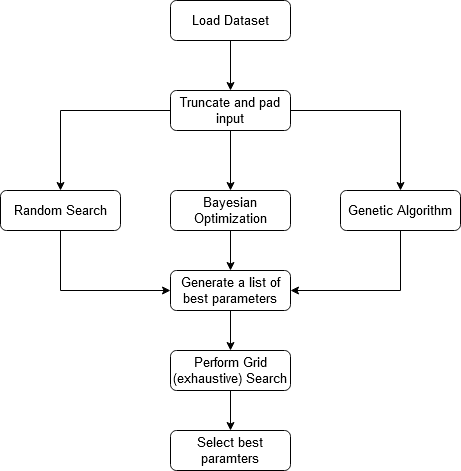
\includegraphics[width=0.5\textwidth, height=10cm, keepaspectratio]{flowchart.png}
\caption{ General workflow which involves loading the dataset, preprocessing, and identification of optimal parameters after going through multiple algorithms. }
 \label{fig:flowchart}
\end{figure}


\begin{table*}[t]
\fontsize{9pt}{11pt}
\selectfont
\centering

\begin{tabular}{|p{4cm}|p{1cm}|p{1.5cm}|p{1.5cm}|p{1.5cm}|p{1cm}|p{1cm}|}
\hline
\multicolumn{1}{|c}{\textbf{Method}} & \multicolumn{4}{|c}{\textbf{Identified Optimum Hyperparameters}}& \multicolumn{1}{|c}{\textbf{AUC}}& \multicolumn{1}{|c|}{\textbf{Time Taken}}\\ 
\hline
\textbf & $\alpha$ & numHidden & numEpochs & maxLength &  & \\
\hline
\textbf{Random Search} & 0.018 & 464 & 5 & 458 & 0.896 & 1h14m\\
\hline
\textbf{Bayesian Optimization} & 0.0031 & 278 & 7 & 422 & 0.9350 & 1h28m\\ 
\hline
\textbf{GA Approach-I} & 0.012 & 54 & 3 & 429 & 0.9378 & 23h30m\\ 
\hline
\textbf{GA Approach-II} & 0.017 & 112 & 4 & 418 & 0.934 & 8h46m\\ 
\hline
\textbf{GA Approach-III} & 0.0075 & 85 & 3 & 475 & 0.946 & 14h22m\\ 
\hline
\textbf{Final Grid Search} & 0.0075 & 85 & 3 & 475 & 0.946 & 7h5m\\
\hline
\end{tabular}%
\label{tab:inference}
\caption{Results and comparison of techniques used. Results were obtained after the model was tested on the test set of $25000$ reviews.}
\label{tab:res}
\end{table*}

\begin{enumerate}
\item Random Search

A set of hyperparameters from the specified range was generated randomly for each iteration and model, and trained on the train set and evaluated on the validation set. We ran $70$ iterations and reported the best set of parameters.


\item Bayesian Optimization

For Bayesian optimization, we use an open-source library, Hyperas\cite{hyperas}. Hyperas uses hyperopt\cite{hyperopt} to do Bayesian optimization. The number of iterations is set at $70$ to make it consistent with random search and see if it offers any advantage in comparison to random search.
\item Genetic Algorithm (GA)
\begin{figure}
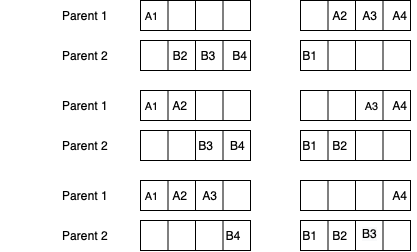
\includegraphics[width=0.4\textwidth, height=8cm, keepaspectratio]{GA.png}
\caption{ Crossover combination for GA }
 \label{fig:ga}
\end{figure}

It starts with a random population of $20$ individuals. Each individual consists of the four hyperparameters. Each individual is represented by its gene encoding. For each individual, we have a $32$ bit to represent its gene. The first $10$ bits are used to encode the learning rate. Note that the bits may go up to $1023$ so we divide it by $2000$ so that the maximum will be equal to $0.51$. Also, in cases when the binary encoding has all zeros, we cap the learning rate to $0.0005$. The minimum of numHidden, numEpochs, and maxLength is capped to $1$.

We perform three different types of experiments using genetic algorithm. Number of population for each generation is $20$ and there are $70$ generations. 

\begin{itemize}
\item Approach-I: For the first generation, each of the $20$ models is run and fitness is calculated for each of them. The fitness for each model is their validation accuracy in the last epoch. The probability \textit{P(M\textsubscript{i})} that determines if a model will be selected as a parent is calculated as
\[
    P(M_i) = \frac{fitness(M_i)^4}{\sum_{n=1}^{20} fitness(M_n)^4}
\] 
The best performing model will be passed on to the next generation and the remaining $19$ are a result of crossover and mutation. Two parents are selected according to the probability described above. We ensure that two parents will not be identical. We use the one-point crossover.
To be more specific, after two parents are selected, a random point is generated which lies between two parents say A and B in the combination of A\textsubscript{1},B\textsubscript{2},B\textsubscript{3},B\textsubscript{4} or A\textsubscript{1},A\textsubscript{2},B\textsubscript{3},B\textsubscript{4} or A\textsubscript{1},A\textsubscript{2},A\textsubscript{3},B\textsubscript{4} or B\textsubscript{1},A\textsubscript{2},A\textsubscript{3},A\textsubscript{4} or B\textsubscript{1},B\textsubscript{2},A\textsubscript{3},A\textsubscript{4} or B\textsubscript{1},B\textsubscript{2},B\textsubscript{3},A\textsubscript{4}.This is represented in Figure \ref{fig:ga}. The production of crossover now has probability of $30$ percent to undergo mutation.

\item Approach-II: Here, we take the top $10$ models from previous generation. We don't need to run the model to get fitness for these top $10$ models which preserves more than one good performing models. It also avoids extra computation. To find the next $10$ we use the same crossover and mutation as described in the first approach.

\item Approach-III: It is essentially similar as the second approach except here we slightly modify the probability \textit{P(M\textsubscript{i})} as \[
    P(M_i) = \frac{fitness(M_i)^2}{\sum_{n=1}^{20} fitness(M_n)^2}
\] The motivation for this approach is to decrease the difference in probability for the top and bottom half of the population. Since we already have the top ten individual from the previous generation, we give higher chance for slightly poor performing models because they could contain an optimal value for one hyperparameter yet is performing poorly due to other hyperparameters. If this optimal parameter is crossed over with other hyperparameters from high performing individuals, this could yield better results. Therefore, we are decreasing our bias on top individuals and exploring more possibilities.

\end{itemize}

\end{enumerate}

\section{Results and Discussions}
For $RQ1$, we looked at the area under the precision-recall curve (AUC) metric to determine the best model. Almost all the methods yielded comparable results, but GA approach-III had the best performance. The random search was the fastest but yielded worse results. We can refer to Table \ref{tab:res} for complete results.


\begin{figure}
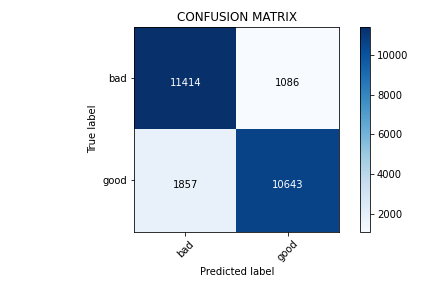
\includegraphics[width=0.5\textwidth, height=10cm, keepaspectratio]{genetic-type-3/genetic-type-3-confusion-matrix.png}
\caption{Confusion matrix for GA approach-III}
 \label{fig:confusion}
\end{figure}
\begin{figure}
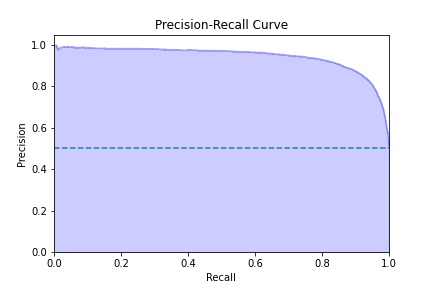
\includegraphics[width=0.5\textwidth, height=10cm, keepaspectratio]{genetic-type-3/Precision-Recall-Curve-genetic-type-3.png}
\caption{PR curve for GA approach-III}
\label{fig:prga}
\end{figure}
\begin{figure}
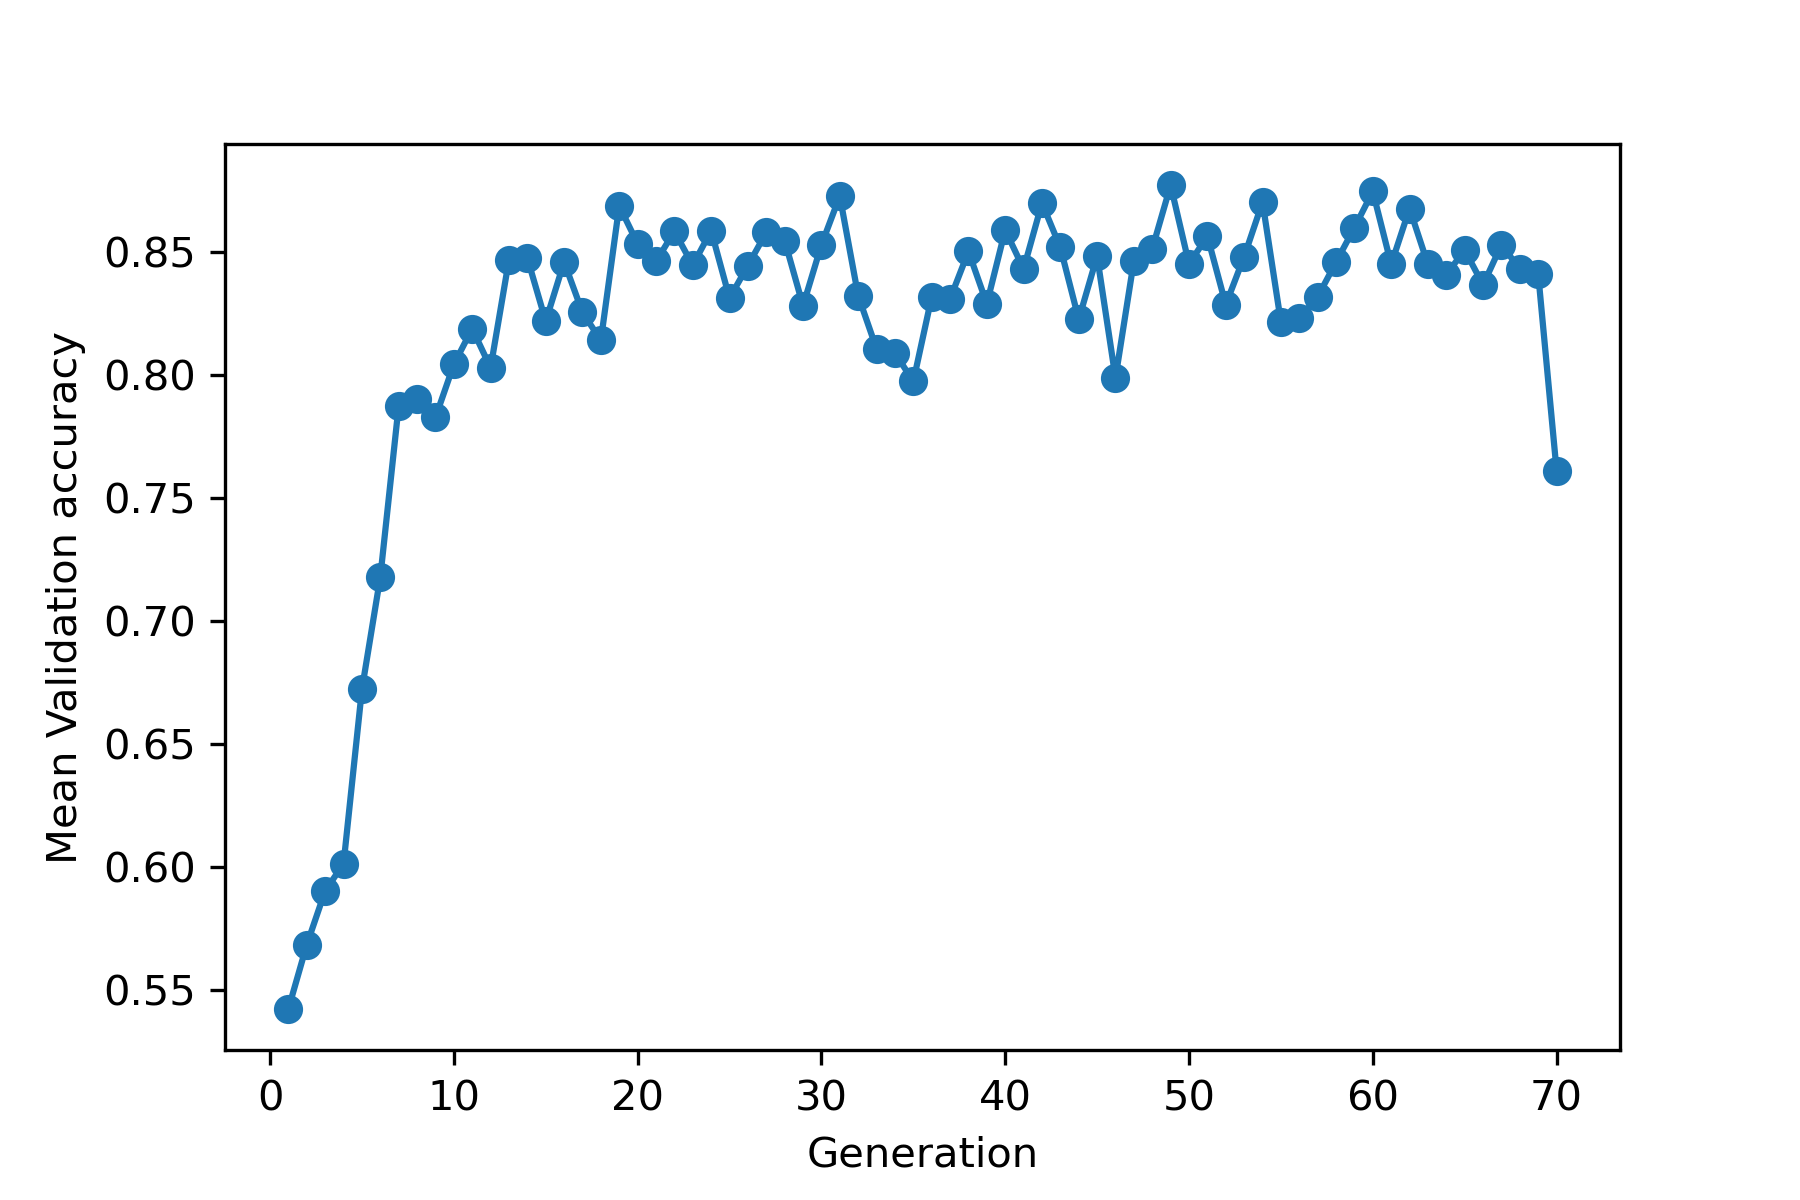
\includegraphics[width=0.5\textwidth, height=10cm, keepaspectratio]{genetic-type-3/genetic-type-3-all-gen.png}
\caption{Improvement of population across generations}
\label{fig:gmv}
\end{figure}

Then we try to answer $RQ2$. Using results from Table \ref{tab:res}, we generate a list of best hyperparameters and fed it to a grid search to determine the best final hyperparameters. We exclude GA approach-II and selected the other two approaches for GA which performed better to reduce the search space for a grid search. The grid search yielded the final parameters which were the same as the ones given by GA approach-III. We were able to obtain an AUC value of $0.946$. Figure \ref{fig:prga} shows the PR curve. For good reviews, the precision was $0.90$, the recall was $0.85$ and the F1 score was $0.88$. Likewise, for bad reviews, the precision was $0.86$, the recall was 0.91 and the F1 score was $0.88$. The grid search took $7$ hours to run.

The GA approach-I ran for $~24$ hours at which point we ran out of memory. We had to save the results for the $35\textsuperscript{th}$ generation and run the algorithm for the next $35$ generation in a new session. The issue arose after the program was run for more than $~14$ hours. We suspect this is a colab notebook issue because we did not run into such problems in GA approach-II or GA approach-III which has almost similar code with only minor modifications which played no part to improve memory usage. 

Figure \ref{fig:gmv} shows how the mean validation accuracy improves  as population evolves. We notice that the mean validation accuracy keeps on rising sharply for the first $15-20$ generations. This shows that the population, in general, are converging towards the solution. However, there is a lot of oscillation after that. This is because even if four or five of the newly formed individuals are poor, they bring down the mean validation accuracy. We remind the reader that we preserve the best models from the previous generation. Even if there is a sharp drop in the $70\textsuperscript{th}$ generation, the best individual in this generation will be the best of this generation and $69\textsuperscript{th}$ generation. This means the best set of parameters is not lost even if there is a drop in mean validation accuracy. Also, there is a possibility that a new model with better parameter may have been formed in $70\textsuperscript{th}$. Hence, we prefer best model of $70\textsuperscript{th}$ generation as the model recommended by GA approach-III.

\section{Conclusion and Future Works}
We were able to tune four core hyperparameters: learning rate, number of hidden units, input length, and the number of epochs in our experiment. Our study shows that GA gives the best result in finding the best model with AUC of $0.946$. Our comparative study between random search, Bayesian optimization, and GA (with grid search) shows that GA gives the optimal hyperparameters with high validation accuracy on the test dataset. However, Random Search and Bayesian Optimization give sub-optimal results with faster training time.

In our experiment, we only selected four hyperparameters. Other hyperparameters such as number of LSTM layers, number of hidden layers, dropout value, optimizer, etc. may be studied as future work. Similar hyperparameter optimization techniques for bidirectional LSTM and bidirectional LSTM with attention could also be future areas of interest. Using Particle Swarm Optimization for searching is another possibility.


\begin{thebibliography}{}


\bibitem{lstm}Hochreiter, S., \& Schmidhuber, J. (1997). Long short-term memory. Neural computation, 9(8), 1735-1780.

\bibitem{hutter}
Hutter, F., Lücke, J., \& Schmidt-Thieme, L. (2015). Beyond Manual Tuning of Hyperparameters. KI - Künstliche Intelligenz, 29(4), 329-337.

\bibitem{bilstm}
Schuster, M., \& Paliwal, K. K. (1997). Bidirectional recurrent neural networks. IEEE transactions on Signal Processing, 45(11), 2673-2681.

\bibitem{batch}
Breuel, T. M. (2015). Benchmarking of LSTM networks. arXiv preprint arXiv:1508.02774.

\bibitem{methods}
Bergstra, J. S., Bardenet, R., Bengio, Y., \& Kégl, B. (2011). Algorithms for hyper-parameter optimization. In Advances in neural information processing systems (pp. 2546-2554).
\bibitem{random}
Bergstra, J., \& Bengio, Y. (2012). Random search for hyper-parameter optimization. Journal of machine learning research, 13(Feb), 281-305.

\bibitem{bayesian}
Snoek, J., Larochelle, H., \& Adams, R. P. (2012). Practical bayesian optimization of machine learning algorithms. In Advances in neural information processing systems (pp. 2951-2959).

\bibitem{optimal}
Reimers, N., \& Gurevych, I. (2017). Optimal hyperparameters for deep lstm-networks for sequence labeling tasks. arXiv preprint arXiv:1707.06799.

\bibitem{melis}
Melis, G., Dyer, C., \& Blunsom, P. (2017). On the state of the art of evaluation in neural language models. arXiv preprint arXiv:1707.05589.
\bibitem{merita}
Merity, S., McCann, B., \& Socher, R. (2017). Revisiting activation regularization for language rnns. arXiv preprint arXiv:1708.01009.

\bibitem{blackbox}
Golovin, D., Solnik, B., Moitra, S., Kochanski, G., Karro, J., \& Sculley, D. (2017, August). Google vizier: A service for black-box optimization. In Proceedings of the 23rd ACM SIGKDD international conference on knowledge discovery and data mining (pp. 1487-1495)

\bibitem{imdb}
Maas, A. L., Daly, R. E., Pham, P. T., Huang, D., Ng, A. Y., \& Potts, C. (2011, June). Learning word vectors for sentiment analysis. In Proceedings of the 49th annual meeting of the association for computational linguistics: Human language technologies-volume 1 (pp. 142-150). Association for Computational Linguistics.

\bibitem{eggen}
Eggensperger, K., Feurer, M., Hutter, F., Bergstra, J., Snoek, J., Hoos, H., \& Leyton-Brown, K. (2013, December). Towards an empirical foundation for assessing bayesian optimization of hyperparameters. In NIPS workshop on Bayesian Optimization in Theory and Practice (Vol. 10, p. 3).

\bibitem{speed}
Chandrashekaran, A., \& Lane, I. R. (2017, September). Speeding up hyper-parameter optimization by extrapolation of learning curves using previous builds. In Joint European Conference on Machine Learning and Knowledge Discovery in Databases (pp. 477-492). Springer, Cham.

\bibitem{hyperas}
M. Pumperla, Hyperas. Github, 2019.

\bibitem{hyperopt}
J. Bergstra, D. Yamins, and D. D. Cox, “Hyperopt: A python library for optimizing the hyperparameters of machine learning algorithms,” in Proceedings of the 12th Python in science conference, 2013, pp. 13–20.

\bibitem{bengio}
Bengio, Y. (2000). Gradient-based optimization of hyperparameters. Neural computation, 12(8), 1889-1900.

\bibitem{weka}
Thornton, C., Hutter, F., Hoos, H. H., \& Leyton-Brown, K. (2013, August). Auto-WEKA: Combined selection and hyperparameter optimization of classification algorithms. In Proceedings of the 19th ACM SIGKDD international conference on Knowledge discovery and data mining (pp. 847-855).

\bibitem{odyssey}
Greff, K., Srivastava, R. K., Koutník, J., Steunebrink, B. R., \& Schmidhuber, J. (2016). LSTM: A search space odyssey. IEEE transactions on neural networks and learning systems, 28(10), 2222-2232.

\bibitem{asha}
Li, L., Jamieson, K., Rostamizadeh, A., Gonina, E., Hardt, M., Recht, B., \& Talwalkar, A. (2018). Massively parallel hyperparameter tuning. arXiv preprint arXiv:1810.05934
\end{thebibliography}

\clearpage
\appendix
\begin{figure}[h!]
\begin{subfigure}{0.5\textwidth}
\centering
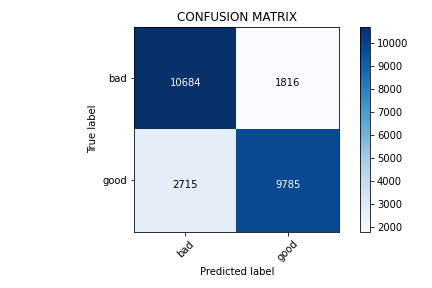
\includegraphics[width=0.95\textwidth]{random/random-confusion-matrix.png}
\caption{Confusion Matrix}
\end{subfigure}%
\begin{subfigure}{0.5\textwidth}
\centering
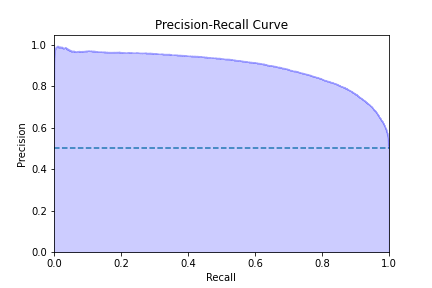
\includegraphics[width=0.95\textwidth]{random/Precision-Recall-Curve-random.png}
\caption{auPRC curve for }
\end{subfigure}%
\caption{Random Search}
\end{figure}


\begin{figure}[h!]
\begin{subfigure}{0.5\textwidth}
\centering
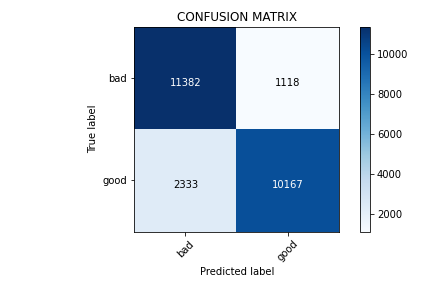
\includegraphics[width=0.95\textwidth]{hyperas/hyperas-confusion-matrix.png}
\caption{Confusion Matrix}
\end{subfigure}%
\begin{subfigure}{0.5\textwidth}
\centering
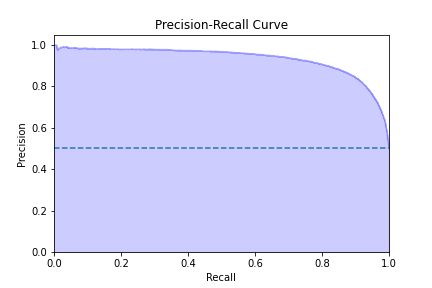
\includegraphics[width=0.95\textwidth]{hyperas/Precision-Recall-Curve-hyperas.png}
\caption{auPRC curve}
\end{subfigure}%
\caption{Bayesian Optimization}
\end{figure}

\begin{figure}[h!]
\centering
\captionsetup{justification=centering}
\begin{subfigure}{0.5\textwidth}
\centering
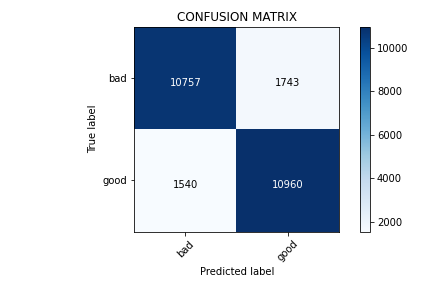
\includegraphics[width=0.95\textwidth]{genetic/bestmodel/genetic-best-confusion-matrix.png}
\caption{Confusion Matrix}
\end{subfigure}%
\begin{subfigure}{0.5\textwidth}
\centering
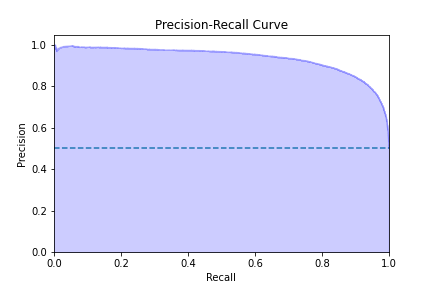
\includegraphics[width=0.95\textwidth]{genetic/bestmodel/genetic-best-recision-Recall-Curve.png}
\caption{auPRC curve}
\end{subfigure}%
\caption{GA approach-I}
\end{figure}


\begin{figure*}[h!]
\begin{subfigure}{0.5\textwidth}
\centering
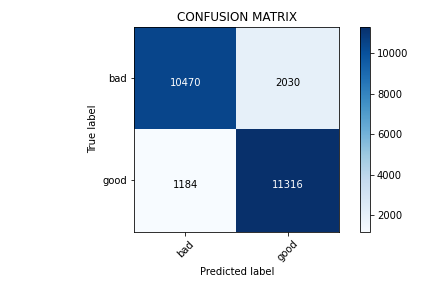
\includegraphics[width=0.95\textwidth]{genetic-type2/genetic-type-2-confusion-matrix.png}
\caption{Confusion Matrix}
\end{subfigure}%
\begin{subfigure}{0.5\textwidth}
\centering
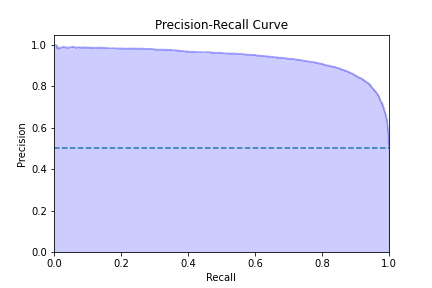
\includegraphics[width=0.95\textwidth]{genetic-type2/Precision-Recall-Curve-genetic-type-2.png}
\caption{auPRC curve}
\end{subfigure}%
\caption{GA approach-II}
\end{figure*}
\end{document}
